\documentclass[main.tex]{subfiles}
\begin{document}
Les signaux déterministe sont utilisé pour les test ou les commandes . Ils sont cependants insuffisant pour décrire l'ensemble des phénomènes qui peuvent être aléatoire ou stochastique. Il est donc nécessaire d'introduire des ``signaux aléatoires'' (SA).
\begin{exemple}[Lot de resistances ``identiques'']
  On considère un lot de résistance de même valeur indiqué par le code couleur, et de même précision. Elles ont en réalité toutes des valeurs différentes $R_i$. on note $s_i(t)$ , la tension au borne de $R_i$.

  On a $s_i(t)=0$ mais avec $A\gg1$ on obtient $A.s_i(t)\neq 0$.

  Alors: $\overline{s_i(t)} = 0$ mais il existe une fluctuation de la tension due au bruit thermique.

  On note alors :
  \[
    s_i(t) = s(t,i) = s(t,\omega)
  \]
  C'est une réalisation particulière du SA, appelé par la suite trajectoire.
\end{exemple}

Dans le cas général on parle de fonction aléatoire $F(\theta,\omega)$ ,où $\theta$ est un paramètre certain (comme le temps par exemple).


\begin{rem}
  Un signal aléatoire n'est caractérisé qu'en moyenne.
  \begin{itemize}
  \item moyenne à $\omega$ donné : $s(t,\omega_0) =s_0(t)$ : \textbf{moyenne temporelle}
  \item moyenne à $t$ donné : $s(t_0,\omega) = s_0(\omega)$ : \textbf{moyenne statistique}.
  \end{itemize}
\end{rem}
On dit aussi que $S(t,\omega) = S_t(\omega)$ est une famille de variable aléaoire indexé par le temps, qui décrit l'aspect incertain à chaque instant.
\begin{figure}[H]
  \centering
  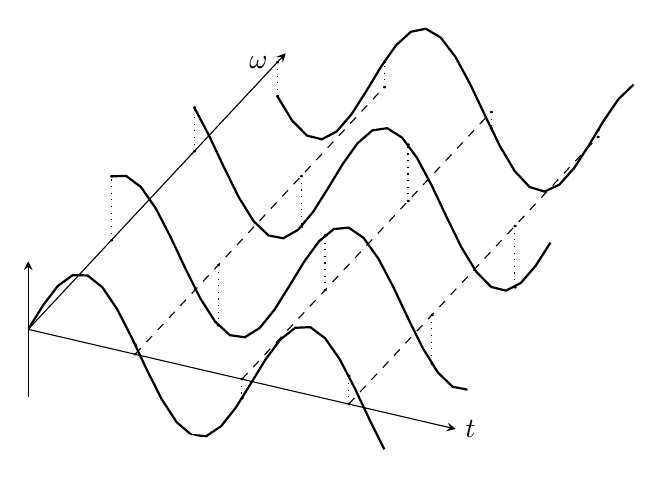
\begin{tikzpicture}
    \begin{axis}[
      scale=1.5,
    axis lines = middle,
    set layers=standard,
    domain=0:10,
    samples y=1,
%   view={-10}{-20},
    unit vector ratio*=1 5 1,
    xtick=\empty, ytick=\empty, ztick=\empty,
    %xlabel=$t$,ylabel=$\omega$,
    xmax=12,ymax=3.1,
    ]
    \foreach \p in {0,1,2,3}
    {\addplot3[thick, black] (x,\p,{2*sin(deg(x)+\p*70)});}
    \foreach \t in {3,6,9}
    {\addplot3[dashed,domain=0:3] (\t,x,0);}
    \foreach \t in {3,6,9}
    \foreach \u in {0,1,2,3}
    {\addplot3[dotted, domain=0:{2*sin(deg(\t)+\u*70)},samples=2,mark size=0.5pt,mark=*] (\t,\u,x);}
    \foreach \v in {1,2,3}
   \addplot3[dotted, domain=0:{2*sin(\v*70)},samples=2,mark size=0.5pt,mark=*] (0,\v,x);
    \node[above,right] at (axis cs: 12,0,0) {$t$};
    \node[above,left] at (axis cs: 0,3,0) {$\omega$};
  \end{axis}
  \end{tikzpicture}
  \caption{Représentation des trajectoires d'un signal aléatoire}
\end{figure}
\end{document}

%%% Local Variables:
%%% mode: latex
%%% TeX-master: "main"
%%% End:
